\chapter{実験}
本章では,提案する視覚エフェクトと振動刺激の提示手法を用いた評価実験を行った.
本章では実験内容及びその結果を示す.

評価実験では,VR上に魔法の杖を表示しそこから特定の形状の魔法を放ち,それに伴いユーザーに対しさまざまな振動刺激を与えた.
これにより魔法の形状に対してどのような振動刺激をユーザーに与えることで,ユーザーの魔法体験感を高めることができるのかを調査した.

\section{実験方法}
本章では作成したシステムを用いた評価実験を行った.
22歳$\sim$24歳の男性8名に対して実験を実施した.

本実験の手順を以下に示す.
手順の2$\sim$4の工程をinceneration,ring-fire,main-beamの順番にそれぞれ繰り返した.
被験者は振動を体験してもらった後,アンケートに回答してもらうので振動パターンを覚えておく必要がある.
その旨を実験説明の段階で被験者に伝えた.

\begin{enumerate}
    \item 実験説明
    \item 実験前アンケート
    \item 実験
    \item 実験後アンケート
\end{enumerate}

\newpage
\section{実験前アンケート}
実験を実施する前にアンケートを行った.

まず,被験者に実験で使用する視覚エフェクトの動画を見せた.
次に視覚エフェクトを時系列順に6分割し並べた画像を被験者に見せた.
それぞれ振動強度がどのように変化しそうであるか,被験者のイメージを手書きでグラフに書いてもらった.
振動強度のグラフを\figref{ank}に示す.

ユーザーが視覚エフェクトに対してどのような振動刺激が与えられるとイメージしているのかを調査した.

\begin{figure}[h]
\centering
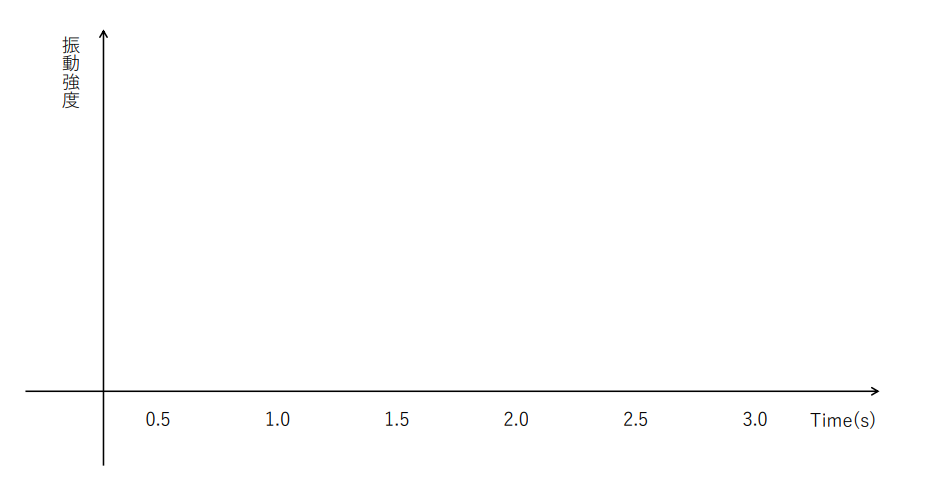
\includegraphics[clip,width=10cm]{./fig/ank.png}
\caption{振動強度のイメージ}\label{ank}
\end{figure}

\section{実験}
被験者はHMDを装着し右手にコントローラーを持つ.
実験の様子を\figref{jikken}に,実験の被験者の視界を\figref{first}に示す.
提示する視覚エフェクトと振動パターンを実験者が選択する.
この時被験者に選択したエフェクトを伝えておく.
視覚エフェクトに対して4パターンの振動刺激を提示した後アンケートを実施した.
これを視覚エフェクトの種類ごとに繰り返した.


実験終了後にアンケートを行う.
実験終了後アンケートでは視覚エフェクトに対しての振動刺激の一致度を5段階で評価してもらった.
評価値1が全く一致していない,評価値5がとても一致しているという評価とした.
システム使用中の没入感やその他気になったことや感想は自由記入形式で回答してもらった.
\begin{figure}[h]
\centering
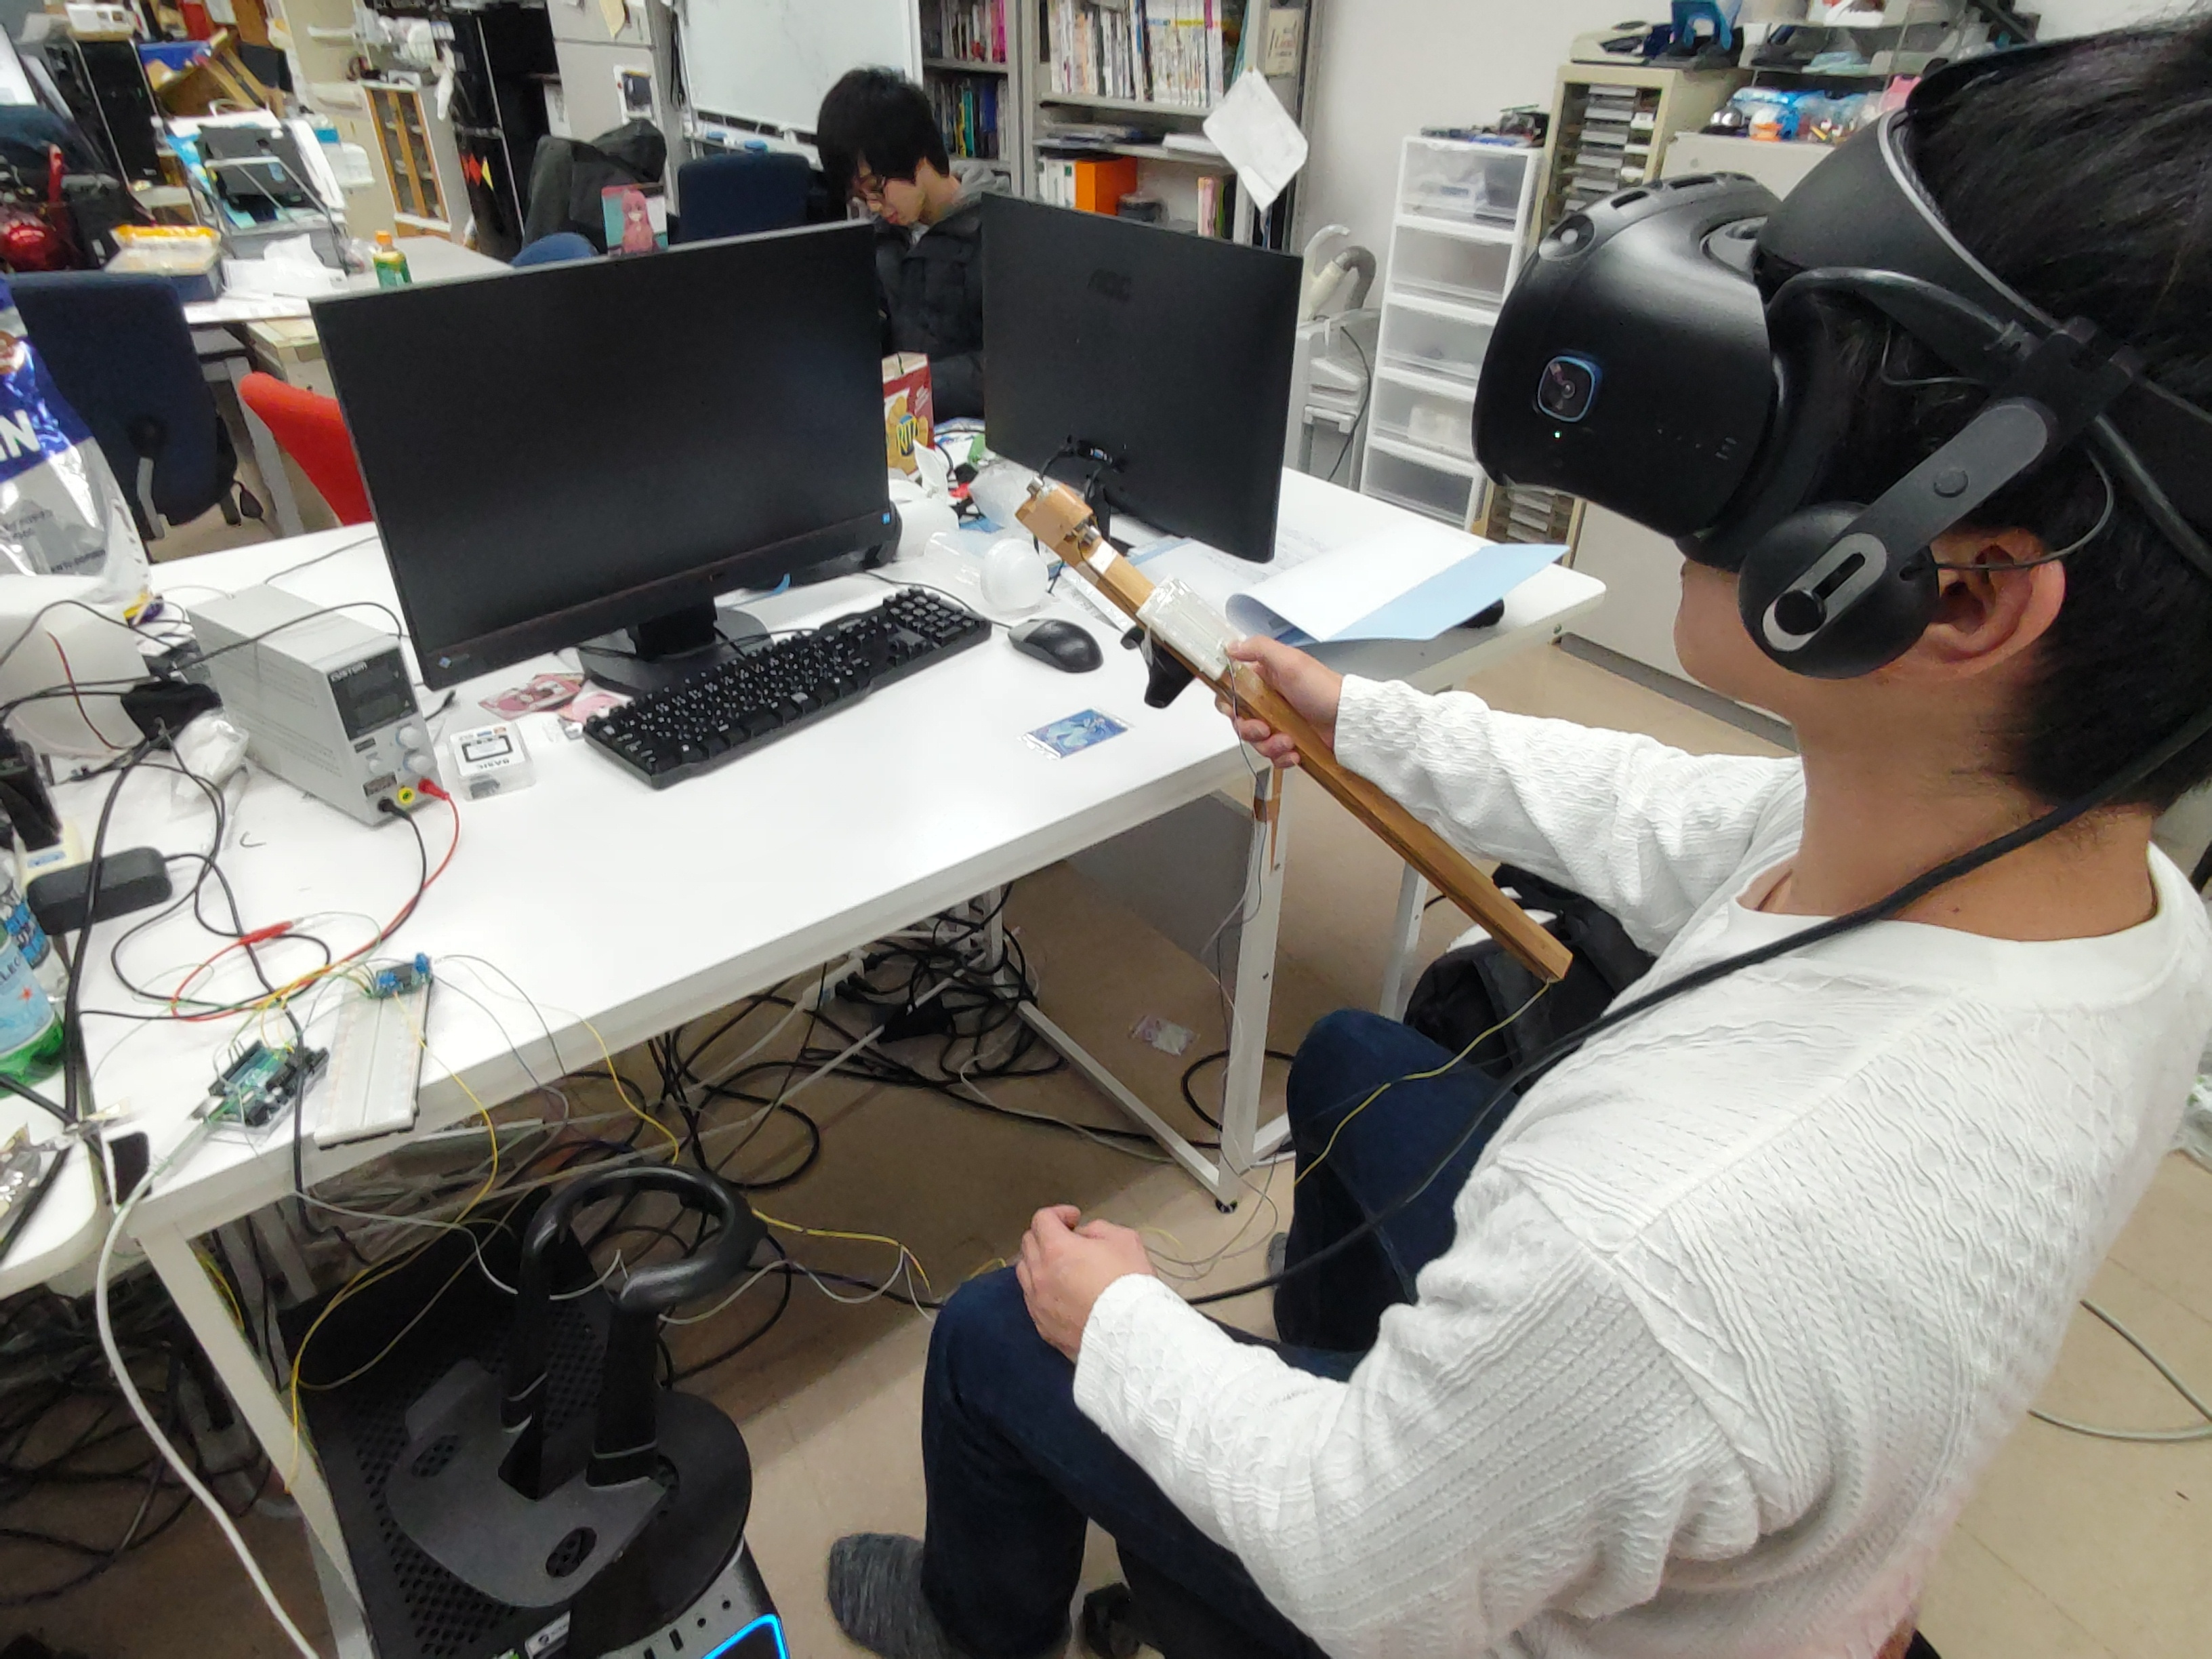
\includegraphics[clip,width=10cm]{./fig/jikken.png}
\caption{実験の様子}\label{jikken}
\end{figure}
\begin{figure}[h]
\centering
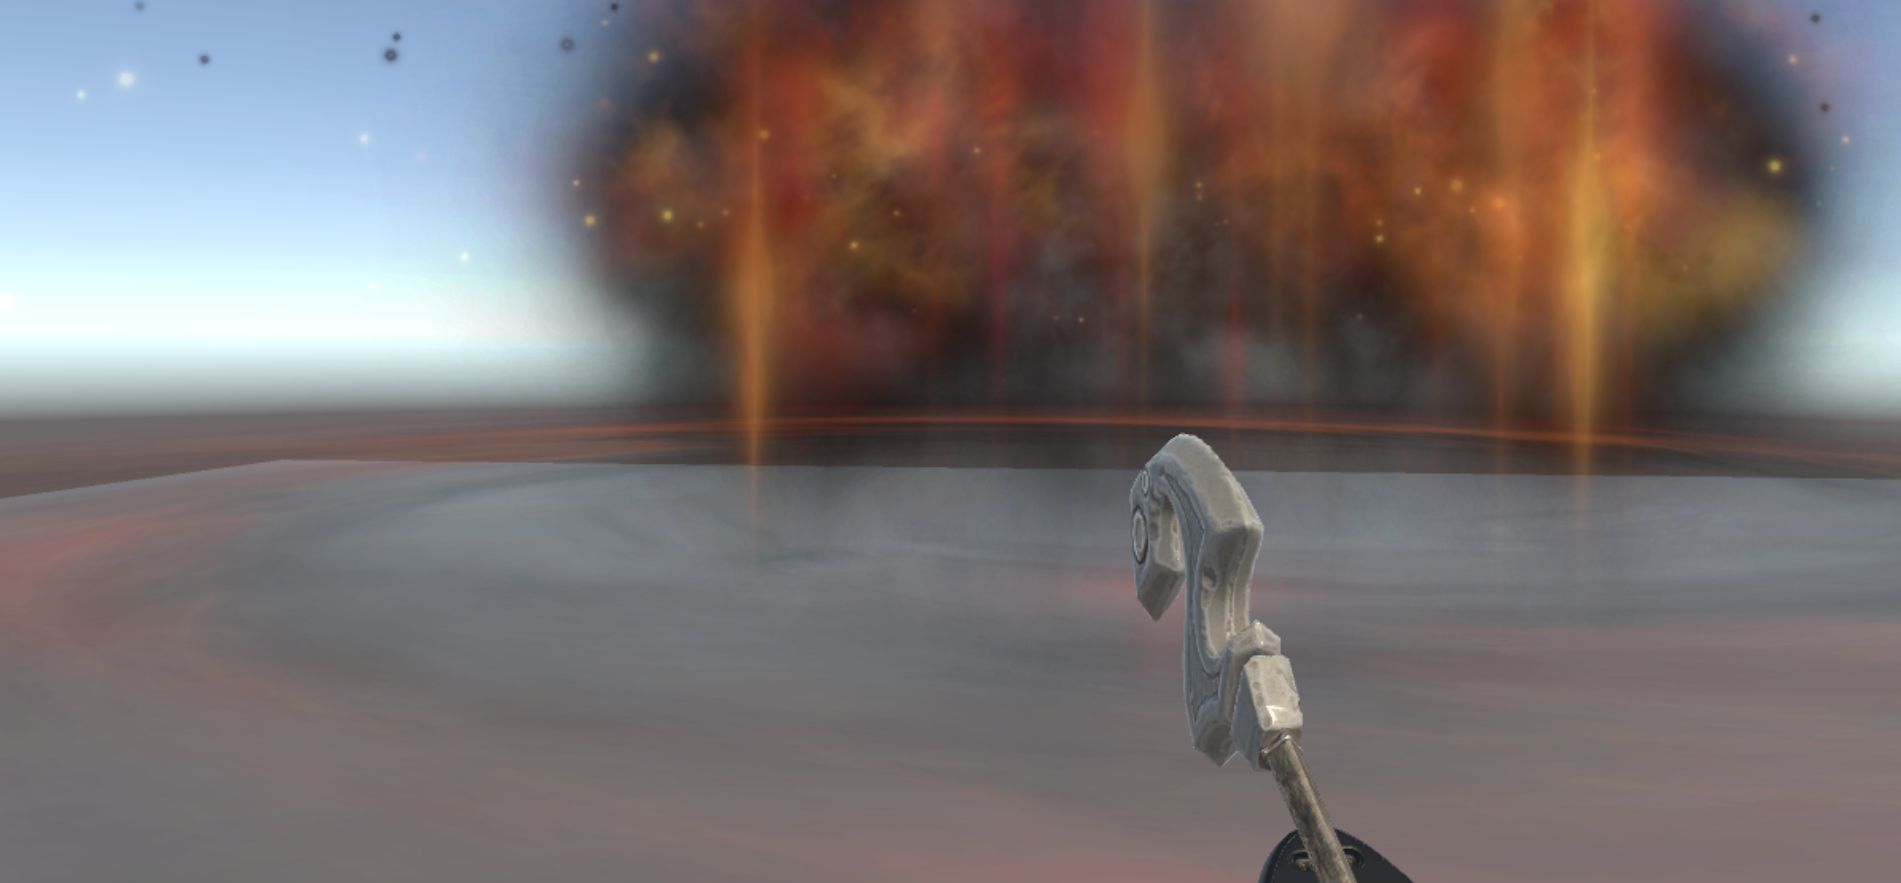
\includegraphics[clip,width=10cm]{./fig/unity.png}
\caption{被験者の視界}\label{first}
\end{figure}


\newpage


\section{結果と考察}
\subsection{実験前アンケート結果}
\figref{inceA}にincenerationについてのアンケート結果を示す.
被験者ほぼ全員がincenerationの振動について,一定であると回答した.
振動パターン1に近い結果となった.

\newpage

\begin{figure}[h]
\centering
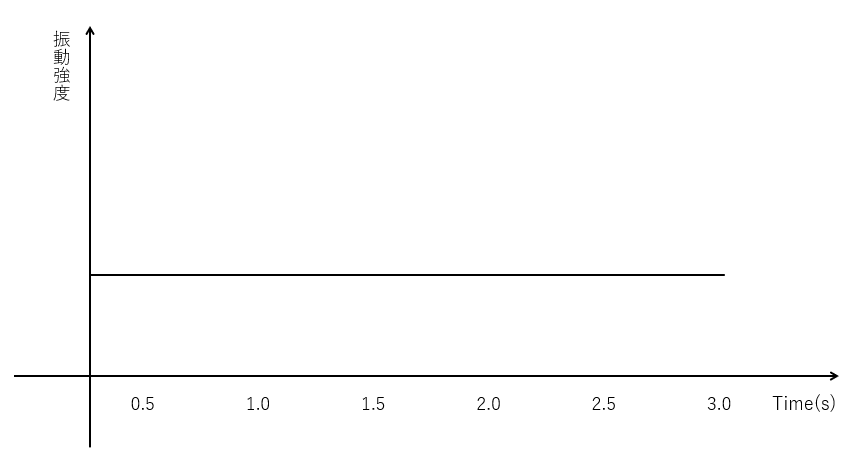
\includegraphics[clip,width=8cm]{fig/incenerationAve.png}
\caption{アンケート結果(inceneration)}\label{inceA}
\end{figure}

\figref{ringA}にring-fireについてのアンケート結果を示す.
2枚目までは小さい振動が続き,3枚目で大きな振動になり,残りは余韻といったイメージであることが分かる.
振動パターン2に近い結果となった.
\begin{figure}[h]
\centering
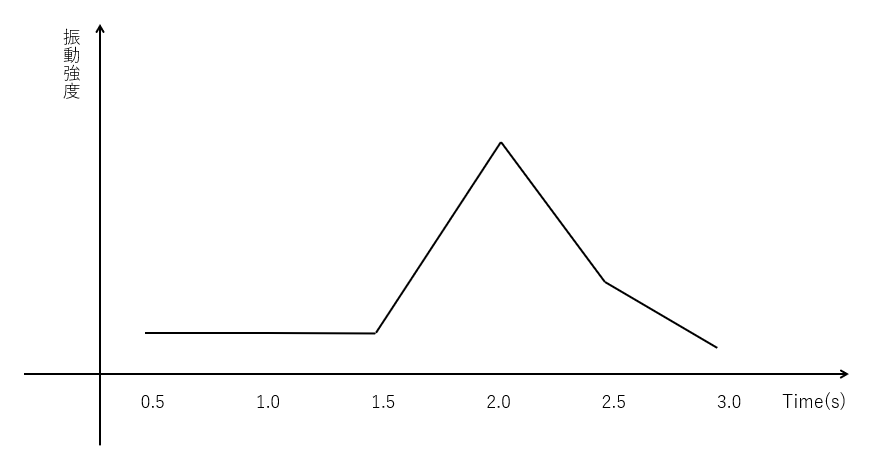
\includegraphics[clip,width=8cm]{fig/ringfireAve.png}
\caption{アンケート結果(ring-fire)}\label{ringA}
\end{figure}



\figref{mainA}にmain-beamについてのアンケート結果を示す.
ring-fireと比較して初めから強い振動があり,残りは余韻といったイメージであることが分かる.
振動パターン3に近い結果となった.
\begin{figure}[h]
\centering
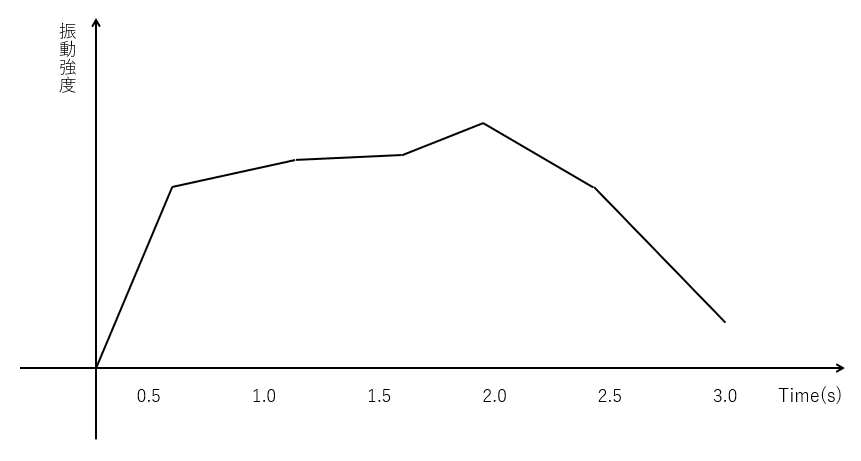
\includegraphics[clip,width=8cm]{fig/mainbeamAve.png}
\caption{アンケート結果(main-beam)}\label{mainA}
\end{figure}


\subsection{実験後アンケート結果}
アンケート結果の5段階評価の平均を求めた.

平均値={(評価値×人数)の評価1$\sim$5までの合計}÷被験者数とした.

\figref{inceAnk}にinceneration,\figref{ringAnk}にring-fire,\figref{mainAnk}にmain-beam体験後のアンケート結果を示す.

\begin{figure}[h]
  \centering
  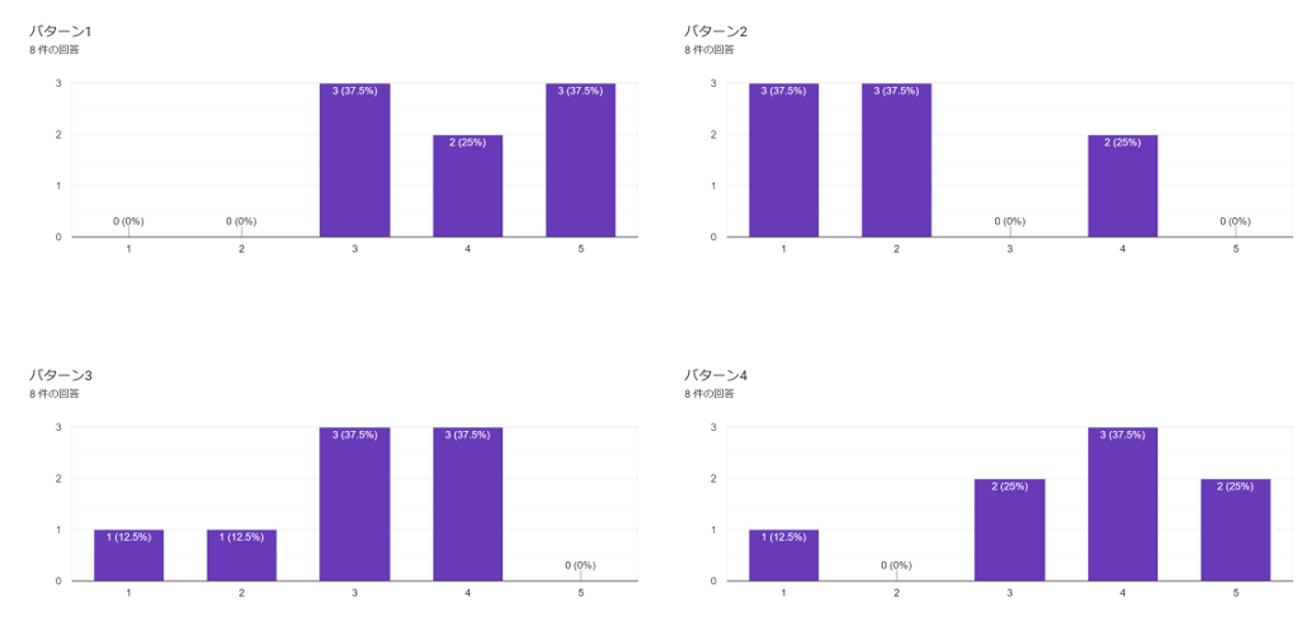
\includegraphics[clip,width=14cm]{./fig/incenerationAnk.png}
  \caption{アンケート結果(inceneration)}\label{inceAnk}
  \end{figure}

\begin{figure}[h]
  \centering
  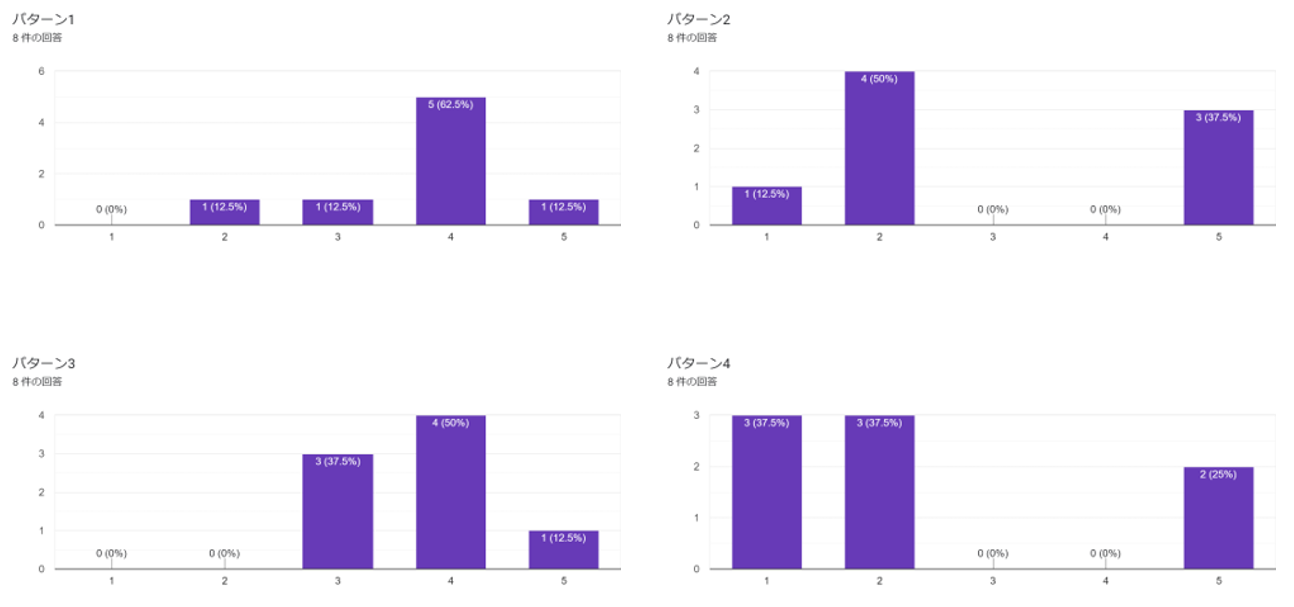
\includegraphics[clip,width=14cm]{fig/ringfireAnk.png}
  \caption{アンケート結果(ring-fire)}\label{ringAnk}
  \end{figure}

\newpage

\begin{figure}[h]
  \centering
  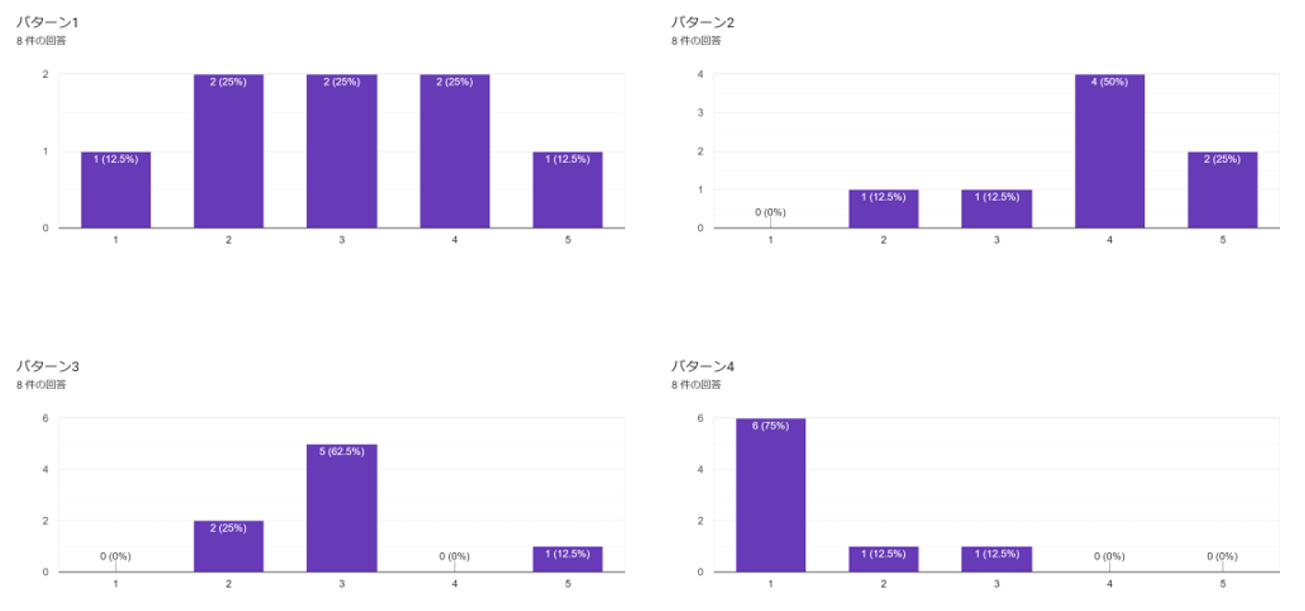
\includegraphics[clip,width=14cm]{fig/mainbeamAnk.png}
  \caption{アンケート結果(main-beam)}\label{mainAnk}
  \end{figure}
  


incenerationのパターンごとの平均を\tabref{tab;inceAvera}に示す.
パターン1の平均の値がほかの振動パターンと比較して,一番高くなっていた.
実験前アンケートの結果と同じ振動パターンの評価が高くなった.
incenerationのような形状の魔法は一定の振動強度の振動フィードバックをユーザーに呈示することで魔法体験感が向上すると考えられる.

\begin{table}[h]
    \caption{平均値(inceneration)}
    \centering
    \begin{tabular}{l|l}
    \hline
    \hline
    振動パターン & 平均値\\
    \hline
    パターン1 & 4\\
    パターン2 & 2.13\\
    パターン3 & 3\\
    パターン4 & 3.63\\
    \hline
    \end{tabular}
    \label{tab;inceAvera}
\end{table}

ring-fireのパターンごとの平均を\tabref{tab;ringAve}に示す.
パターン1とパターン3の平均の値が,他の振動パターンに比べて高かった.
ring-fireのような形状の魔法は,時間推移で徐々に振動強度が強くなる振動フィードバックをユーザーに呈示することで魔法体験感が向上すると考えられる.

\begin{table}[h]
    \caption{平均値(ring-fire)}
    \centering
    \begin{tabular}{l|l}
    \hline
    \hline
    振動パターン & 平均値\\
    \hline
    パターン1 & 3.75\\
    パターン2 & 3\\
    パターン3 & 3.75\\
    パターン4 & 2.38\\
    \hline
    \end{tabular}
    \label{tab;ringAve}
\end{table}

main-beamのパターンごとの平均を\tabref{tab;mainAve}に示す.
パターン2の平均の値が,他の振動パターンに比べて高かった.
ring-fireのような形状の魔法は,時間推移で徐々に振動強度が弱くなる振動フィードバックをユーザーに呈示することで魔法体験感が向上すると考えられる.


  \begin{table}[H]
    \caption{平均値(main-beam)}
    \centering
    \begin{tabular}{l|l}
    \hline
    \hline
    振動パターン & 平均値\\
    \hline
    パターン1 & 3\\
    パターン2 & 3.88\\
    パターン3 & 3\\
    パターン4 & 1.38\\
    \hline
    \end{tabular}
    \label{tab;mainAve}
\end{table}

事前アンケートの結果と同じような振動パターンの評価が高くなる傾向にあった.

ユーザーは視覚エフェクトが大きくなるタイミングで振動も大きくなることで,視覚エフェクトと振動刺激が一致しているように感じると考えられる.


